\section{Understanding the GUI of Scilab}

	\subsection{Panes and layout}
		The layout of Scilab's GUI is divided into five distinct panes, each of which has its own unique functionality.
		\begin{enumerate}
			\item \textit{File browser} -- allows one to browse through the directory tree to easily navigate to the relevant Scilab script file or folder containing the same. 
			\begin{figure}[!htb]
				\centering
				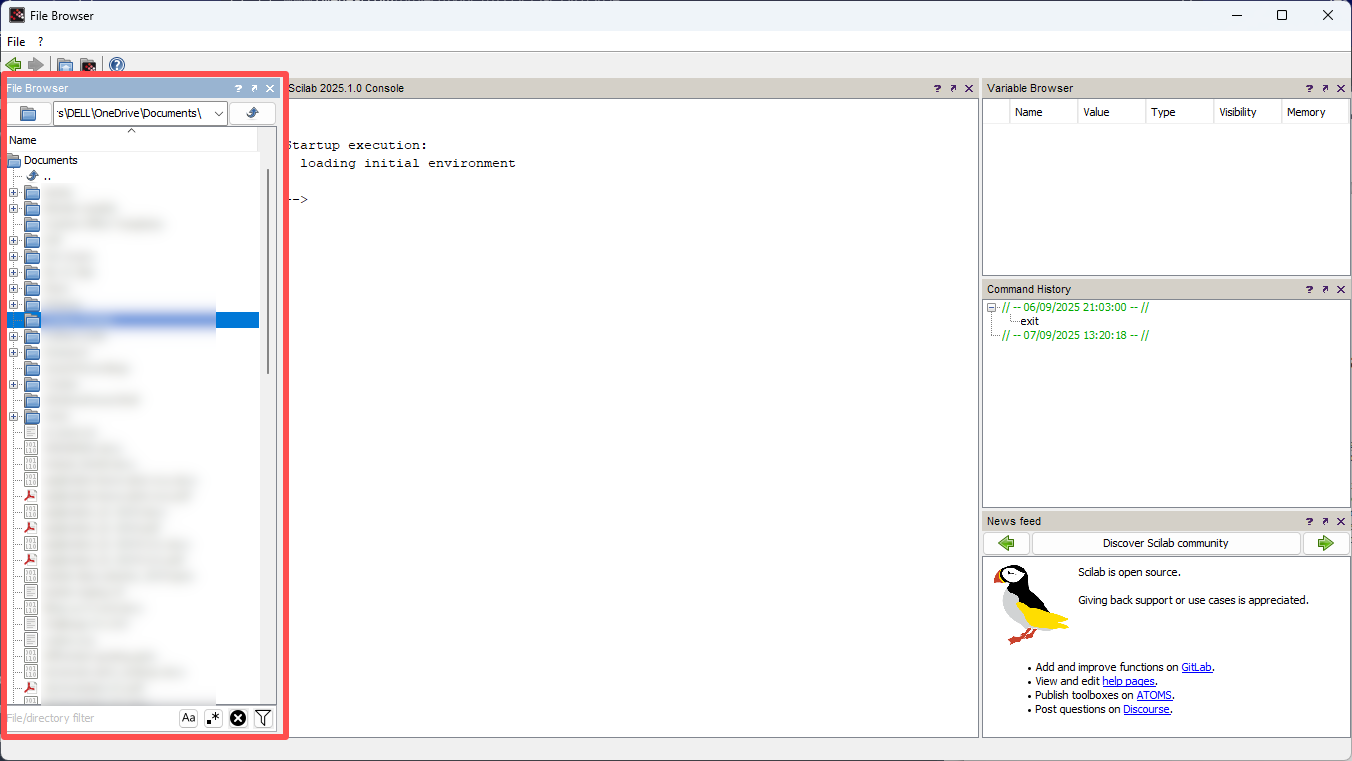
\includegraphics[width=0.9\linewidth]{figures/gui/fig_file-browser.png}
			\end{figure}
			
			\item \textit{Console window} -- allows one to type and execute Scilab commands, as well as to view the output.
			\begin{figure}[!htb]
				\centering
				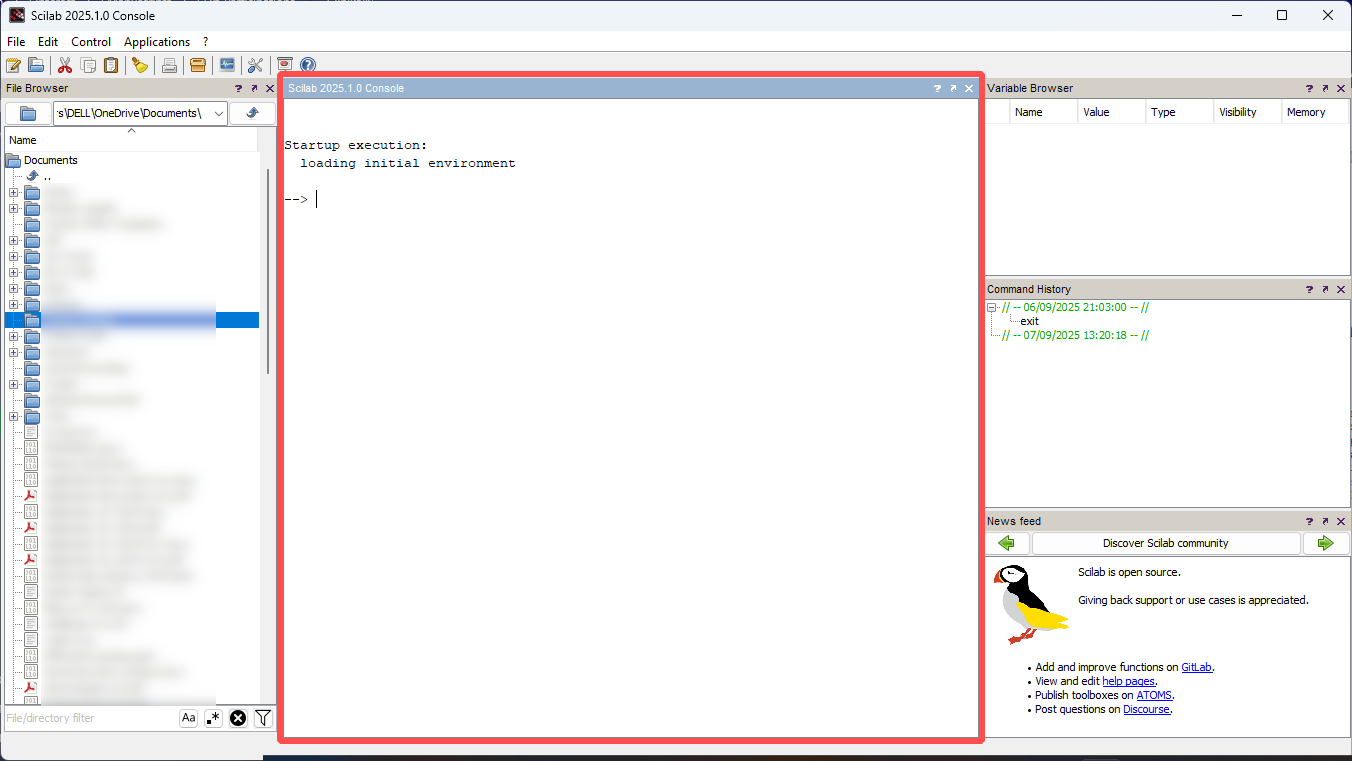
\includegraphics[width=0.9\linewidth]{figures/gui/fig_console.png}
			\end{figure}
			
			\newpage
			\item \textit{Variable browser} -- displays all the variable that have been created by Scilab and are currently active in memory locations.
			\begin{figure}[!htb]
				\centering
				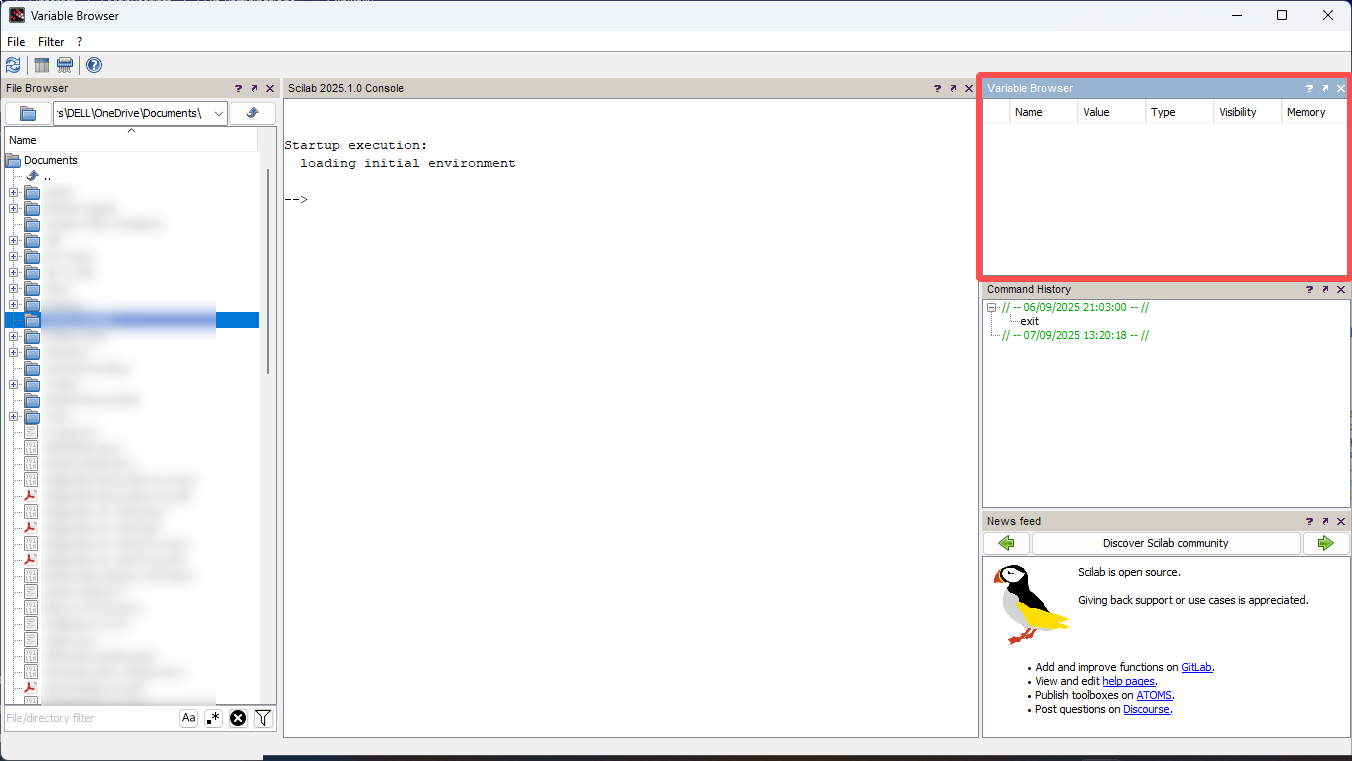
\includegraphics[width=0.9\linewidth]{figures/gui/fig_variable-browser.png}
			\end{figure}
			
			\item \textit{Command history} -- display a chronological order of all the Scilab commands executed by the user, with the most recent command being at the top.
			\begin{figure}[!htb]
				\centering
				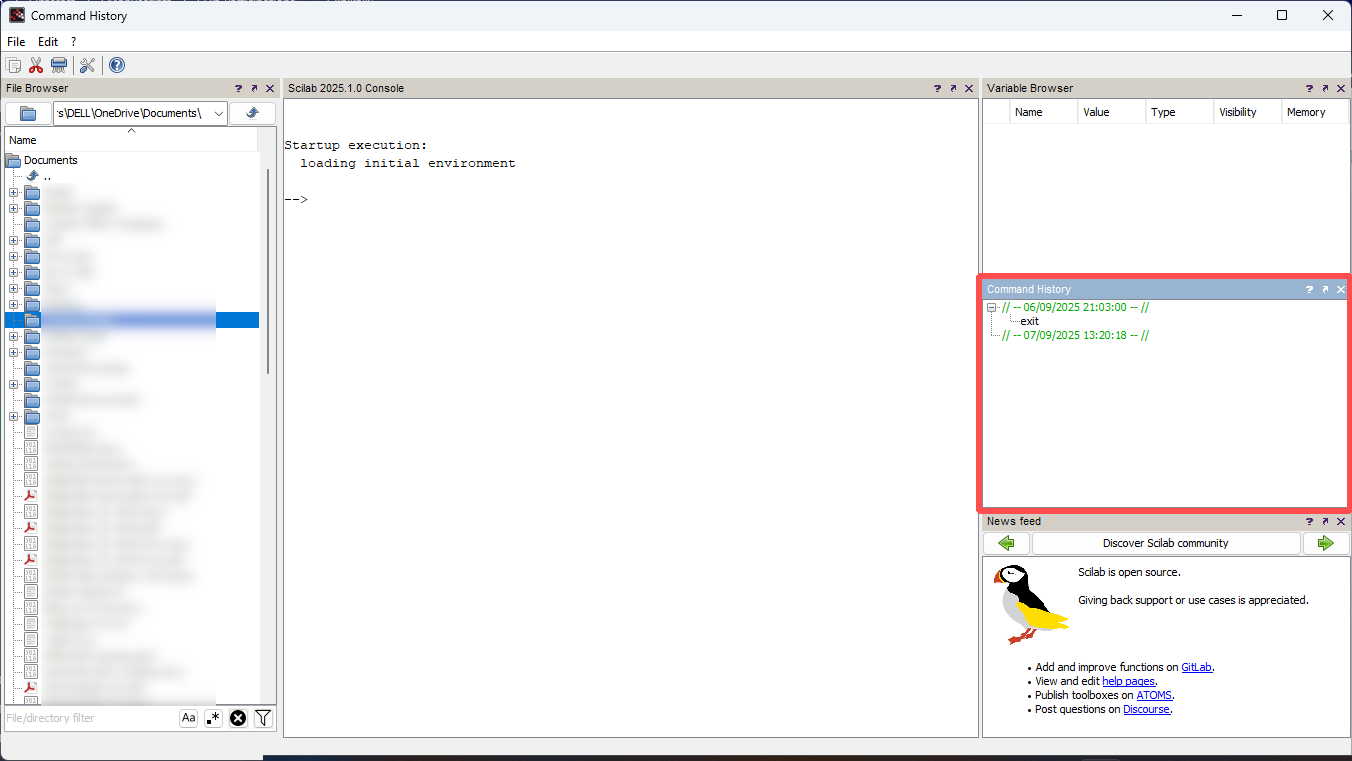
\includegraphics[width=0.9\linewidth]{figures/gui/fig_command-history.png}
			\end{figure}
			
			\newpage
			\item \textit{News feed} -- provides Scilab news and an interface to interact with the online Scilab community.
			\begin{figure}[!htb]
				\centering
				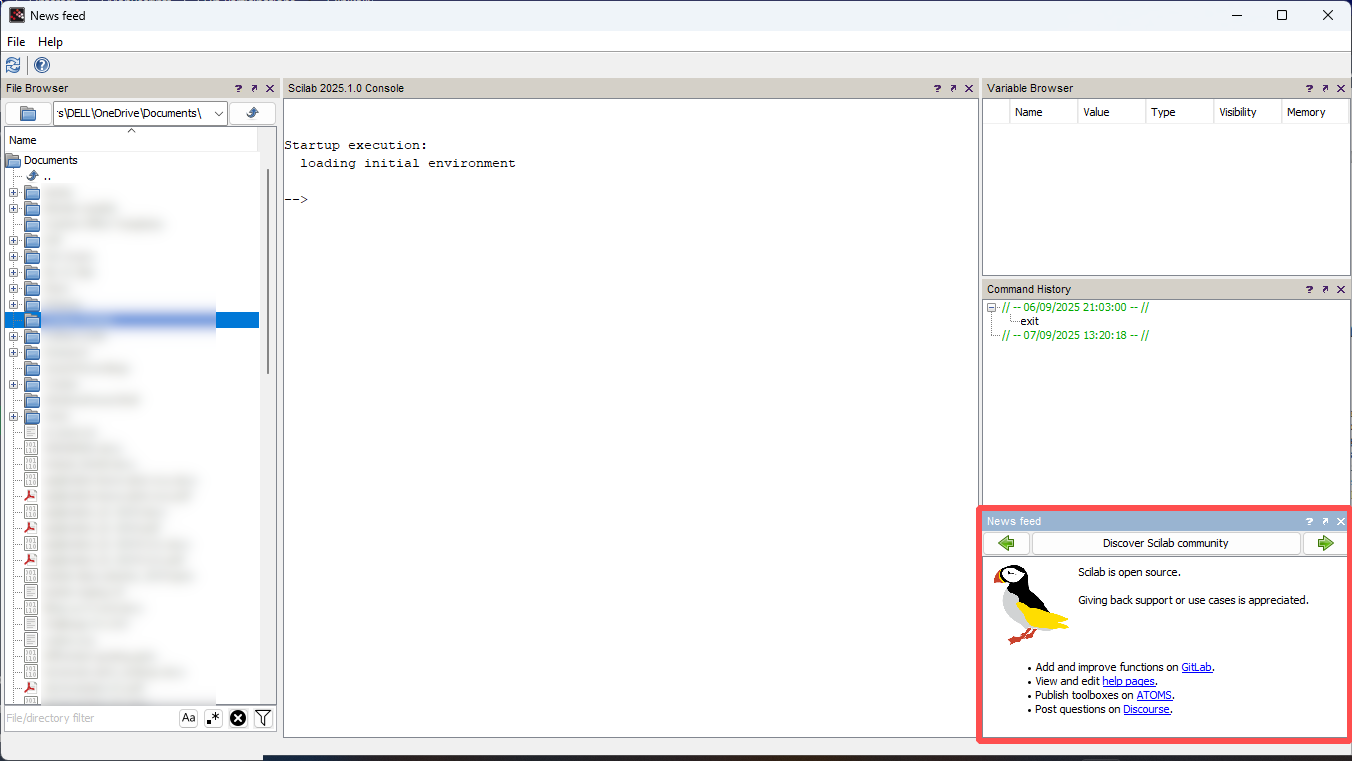
\includegraphics[width=0.9\linewidth]{figures/gui/fig_news-feed.png}
			\end{figure}
		\end{enumerate}
	
	\subsection{The Workspace} \label{ssec:scilab-workspace}
		The Scilab workspace consists of the following components:
		\begin{enumerate}
			\item \textbf{The console window}
			\begin{itemize}
				\item Docked on the GUI by default.
				\item One can perform numerical calculations right from the console and view the output as soon as the computations are complete.
				\item One can find the current directory that one is working on by using the command \texttt{pwd} (which stands for \textit{\textbf{p}resent \textbf{w}orking \textbf{d}irectory}) on the console window.
				\item The Scilab console presents a full-featured, interactive, command-line REPL (\textit{read-evaluate-print-loop}) shell.
				% Essentially the Scilab command prompt does the following:
				% \begin{itemize}
					%     \item \textit{\textbf{R}eads} what a user types
					%     \item \textit{\textbf{E}valuates} what it reads
					%     \item \textit{\textbf{P}rints} out the return value after evaluation
					%     \item \textit{\textbf{L}oops} back and does it all over again
					% \end{itemize}
			\end{itemize}
			\item \textbf{The variable browser}
			\begin{itemize}
				\item Docked on the GUI by default.
				\item One can view the names of the variables, the value they store as well as the memory they are allocated.
			\end{itemize}
			\item \textbf{The command history}
			\begin{itemize}
				\item Docked on the GUI by default.
				\item One can click on any of the earlier commands from the command history to re-run the same without having to type the command all over again.
			\end{itemize}
			\item \textbf{The SciNotes editor}: Running multiple lines of command is not possible on the console window. Also, the console window does not allow one to save a program such that it can be executed later. For these reasons, Scilab provides its own editor, known as SciNotes, that allow the user to write and save multi-line programs that can be executed at any point of time on any other PC with Scilab installed.
			\begin{itemize}
				\item Not docked on the GUI by default.
				\item To open SciNotes, one can either click on its icon on the taskbar (as shown in figure \ref{fig:scinotes-taskbar}), or one can use the main menu by clicking \texttt{Applications} $\rightarrow$ \texttt{SciNotes} (as shown in figure \ref{fig:scinotes-menu}).
			\end{itemize}
			\begin{figure}[!h]
				\centering
				\begin{subfigure}[b]{0.45\textwidth}
					\centering
					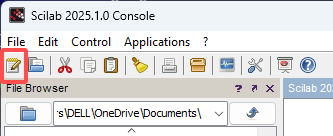
\includegraphics[width=0.8\textwidth,frame]{figures/gui/fig_scinotes-taskbar.png}
					\caption{Opening SciNotes using the taskbar icon}
					\label{fig:scinotes-taskbar}
				\end{subfigure}
				\hfill
				\begin{subfigure}[b]{0.45\textwidth}
					\centering
					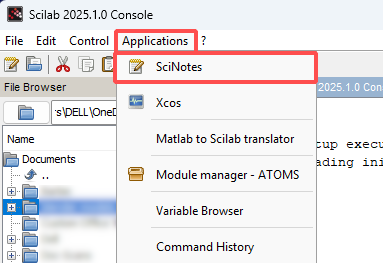
\includegraphics[width=0.8\textwidth,frame]{figures/gui/fig_scinotes-menu.png}
					\caption{Opening SciNotes using the main menu}
					\label{fig:scinotes-menu}
				\end{subfigure}
				\caption{Two ways to open SciNotes}
				\label{fig:scinotes}
			\end{figure}
			\item \textbf{The graphic window}: The graphic window is used for displaying any graphical output, such as the plot resulting from a numerical computation or a simulation result.
			\begin{itemize}
				\item Not docked on the GUI by default.
				\item A graphical window opens up automatically when making any plot.
				\item A graphical window may be opened by running any of the plot commands in Scilab either from the console window or by including it as a line in a Scilab program written using SciNotes.
				\item One can view a generic sample plot using a graphical window by simply typing \texttt{plot} on the console window, as illustrated in figure \ref{fig:generic-plot}.
				\begin{figure}[!htb]
					\centering
					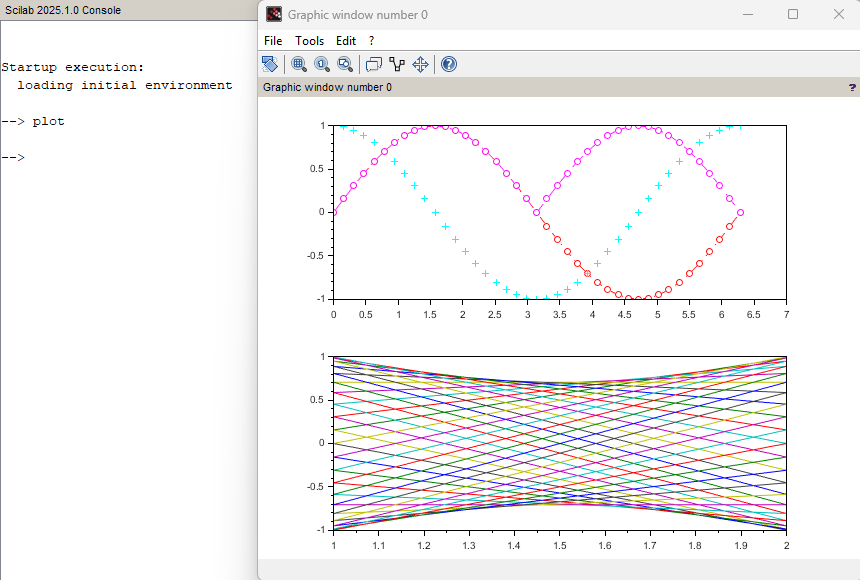
\includegraphics[width=0.5\linewidth,frame]{figures/fig_generic-plot.png}
					\caption{Generic sample plot on a graphical window}
					\label{fig:generic-plot}
				\end{figure}
			\end{itemize}
		\end{enumerate}
	
	\subsection{Documentation and help}
		Scilab provides plenty of resources in the form of documentation that can be easily accessed from the main menu by clicking \texttt{?}. We are primarily interested in two of the sub-menu items, namely \texttt{Scilab Help} (which can be directly accessed by pressing the F1 key) and \texttt{Scilab Demonstrations}, as illustrated in figure \ref{fig:documentation}.
		\begin{figure}[!htb]
			\centering
			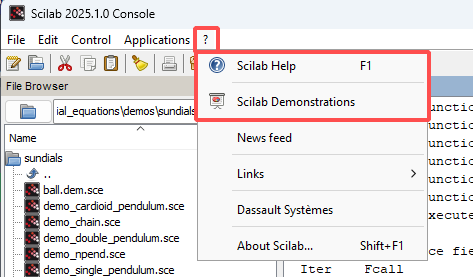
\includegraphics[width=0.6\linewidth]{figures/fig_scilab-documentation.png}
			\caption{Documentation in Scilab}
			\label{fig:documentation}
		\end{figure}
		
		\begin{itemize}
			\item \textbf{Scilab Help}: The Scilab Help Browser window provides detailed documentation on all the features and functions provided in various toolboxes that come bundled with Scilab.
			
			One can either navigate to the exact topic using the hierarchical directory tree structure, or one may search for the specific topic of interest.
			\begin{figure}[!htb]
				\centering
				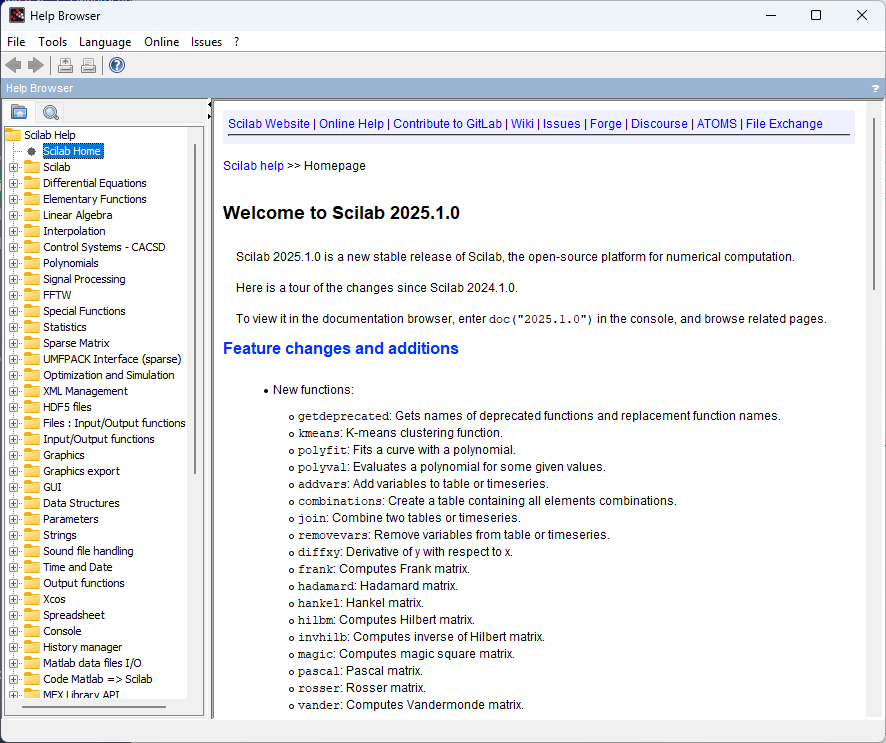
\includegraphics[width=0.6\linewidth]{figures/fig_scilab-help.png}
				\caption{Scilab help browser window}
				\label{fig:doc-help}
			\end{figure}
			
			\item \textbf{Scilab Demonstrations}: Scilab provides a collection of demonstration scripts, which are available on the demonstrations menu. In figure \ref{fig:doc-demos}, an example is displayed as to how one can access a particular demonstration, in this case by clicking \texttt{Simulation} $\rightarrow$ \texttt{ODE's} $\rightarrow$ \texttt{Lorenz equation} from the demonstrations menu. This would open up a graphic window where the demonstration is performed. One can also view the underlying Scilab code by clicking on \texttt{-}\texttt{- View Code -}\texttt{-} on the main menu of the same graphic window.
			
			\begin{figure}[!htb]
				\centering
				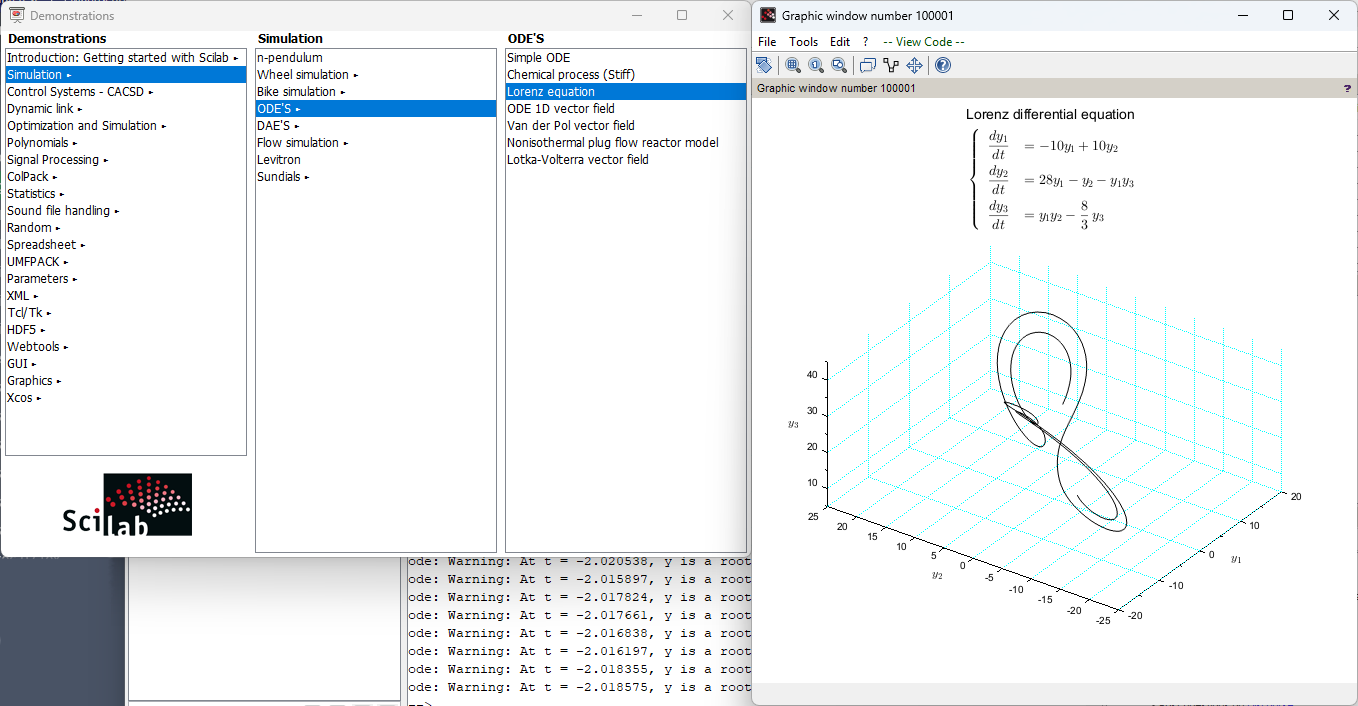
\includegraphics[width=0.9\linewidth]{figures/fig_scilab-demos.png}
				\caption{Scilab help browser window}
				\label{fig:doc-demos}
			\end{figure}
		\end{itemize}